\documentclass[9pt]{article}
\usepackage[margin=0.35in,landscape]{geometry}
\usepackage{tikz}
\usepackage{adjustbox}
\usetikzlibrary{arrows.meta}
\pagestyle{empty}
\begin{document}
\begin{center}
{\Large \textbf{Week 08 Round 3 Agent Architecture -- 25512084}}\\[-1mm]
{\small Custom seller, buyer, persistent memory, and demand-driven restocking around the course runtime}
\end{center}
\vspace{-1mm}

\begin{adjustbox}{max totalsize={0.98\textwidth}{0.80\textheight},center}
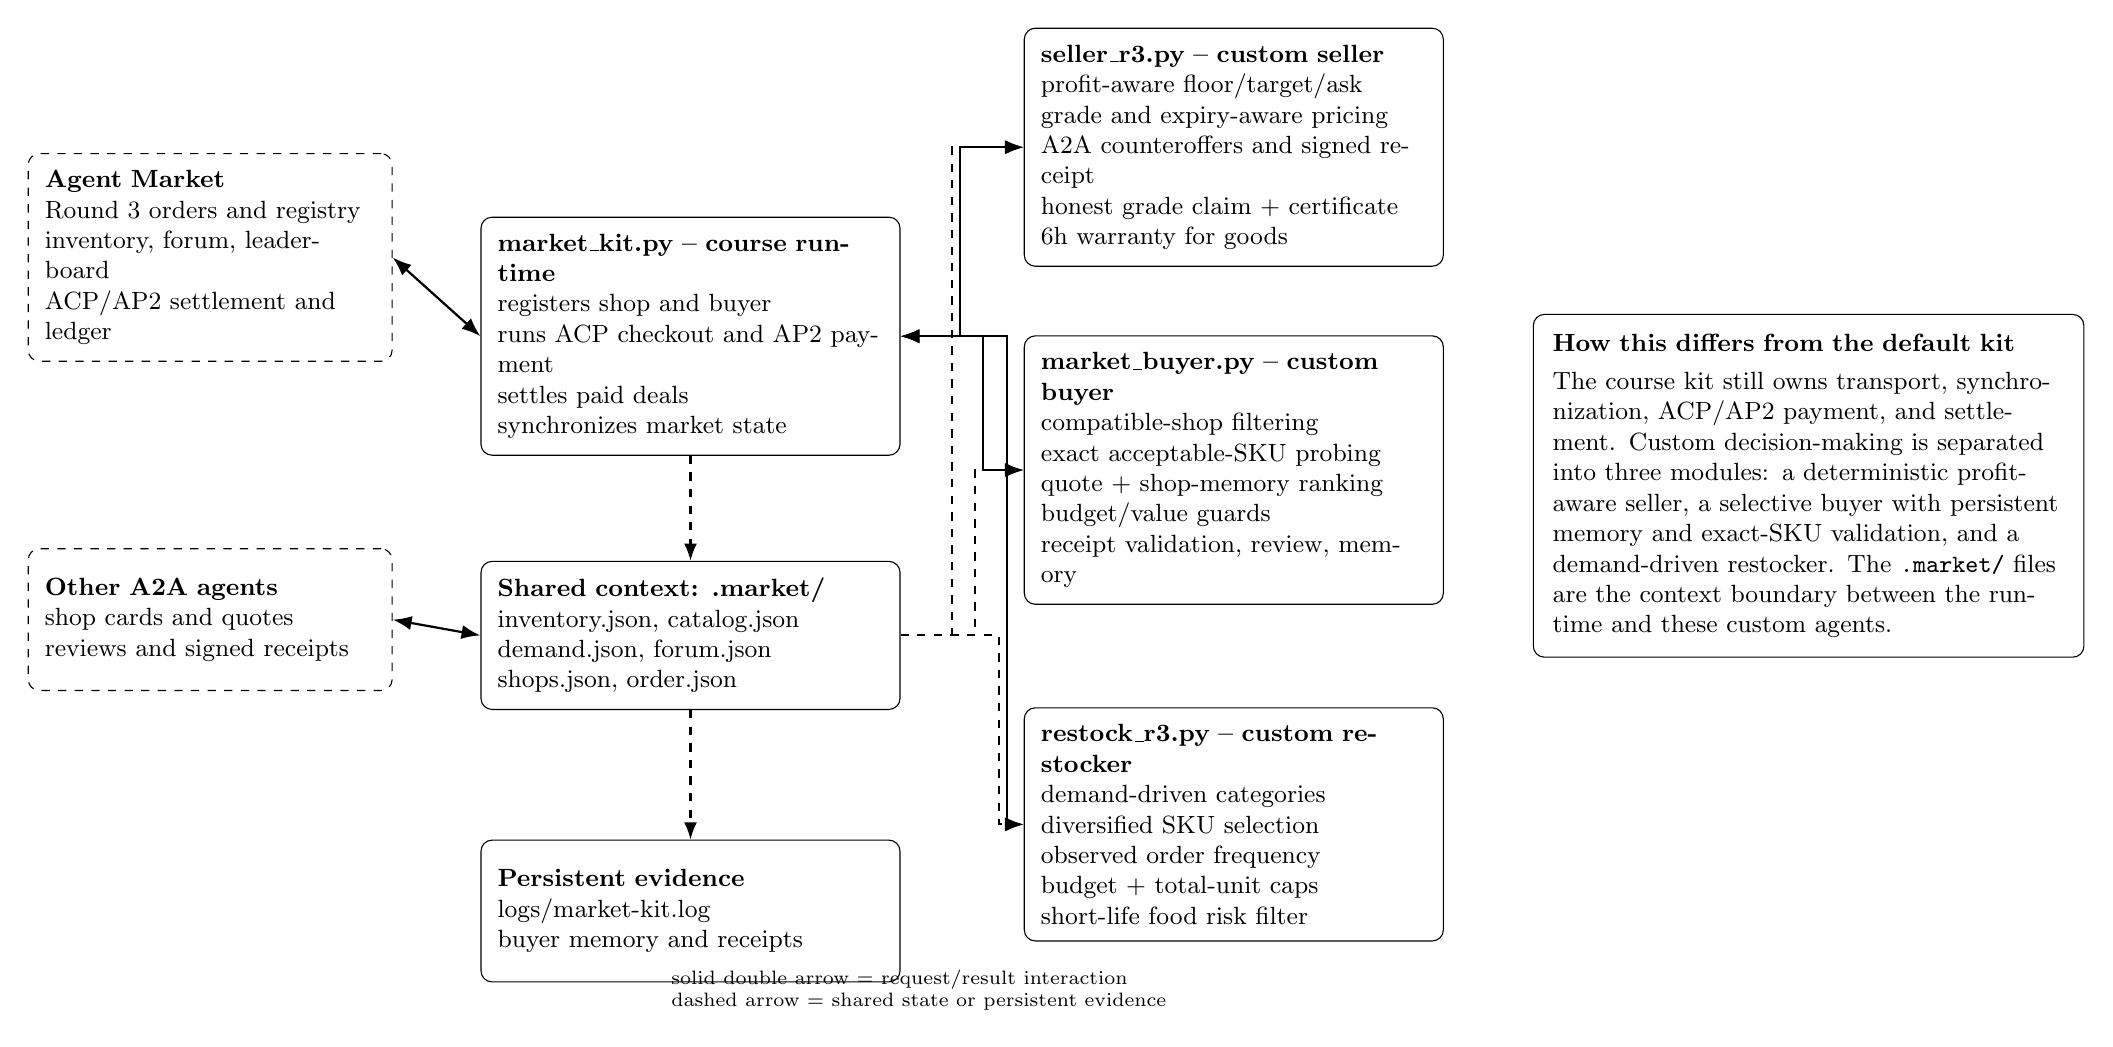
\begin{tikzpicture}[
 font=\small,
 box/.style={draw, rounded corners, align=left, inner sep=6pt, text width=49mm, minimum height=18mm},
 ext/.style={draw, dashed, rounded corners, align=left, inner sep=6pt, text width=42mm, minimum height=18mm},
 note/.style={draw, rounded corners, align=left, inner sep=7pt, text width=65mm, minimum height=25mm},
 flow/.style={-{Latex[length=2.4mm]}, line width=0.8pt},
 both/.style={{Latex[length=2.4mm]}-{Latex[length=2.4mm]}, line width=0.8pt},
 data/.style={-{Latex[length=2.2mm]}, dashed, line width=0.75pt}
]

\node[ext] (market) at (0,3.1) {\textbf{Agent Market}\\Round 3 orders and registry\\inventory, forum, leaderboard\\ACP/AP2 settlement and ledger};
\node[ext] (peers) at (0,-1.5) {\textbf{Other A2A agents}\\shop cards and quotes\\reviews and signed receipts};

\node[box] (kit) at (6.1,2.1) {\textbf{market\_kit.py -- course runtime}\\registers shop and buyer\\runs ACP checkout and AP2 payment\\settles paid deals\\synchronizes market state};
\node[box] (ctx) at (6.1,-1.7) {\textbf{Shared context: .market/}\\inventory.json, catalog.json\\demand.json, forum.json\\shops.json, order.json};
\node[box] (evidence) at (6.1,-5.2) {\textbf{Persistent evidence}\\logs/market-kit.log\\buyer memory and receipts};

\node[box] (seller) at (13.0,4.5) {\textbf{seller\_r3.py -- custom seller}\\profit-aware floor/target/ask\\grade and expiry-aware pricing\\A2A counteroffers and signed receipt\\honest grade claim + certificate\\6h warranty for goods};
\node[box] (buyer) at (13.0,0.4) {\textbf{market\_buyer.py -- custom buyer}\\compatible-shop filtering\\exact acceptable-SKU probing\\quote + shop-memory ranking\\budget/value guards\\receipt validation, review, memory};
\node[box] (restock) at (13.0,-4.1) {\textbf{restock\_r3.py -- custom restocker}\\demand-driven categories\\diversified SKU selection\\observed order frequency\\budget + total-unit caps\\short-life food risk filter};

\node[note] (delta) at (20.3,0.2) {\textbf{How this differs from the default kit}\\[1mm]
The course kit still owns transport, synchronization, ACP/AP2 payment, and settlement. Custom decision-making is separated into three modules: a deterministic profit-aware seller, a selective buyer with persistent memory and exact-SKU validation, and a demand-driven restocker. The \texttt{.market/} files are the context boundary between the runtime and these custom agents.};

% External interactions
\draw[both] (market.east) -- (kit.west);
\draw[both] (peers.east) -- (ctx.west);

% Runtime state and evidence
\draw[data] (kit.south) -- (ctx.north);
\draw[data] (ctx.south) -- (evidence.north);

% Runtime invokes custom modules
\draw[both] (kit.east) -- ++(0.75,0) |- (seller.west);
\draw[both] (kit.east) -- ++(1.05,0) |- (buyer.west);
\draw[both] (kit.east) -- ++(1.35,0) |- (restock.west);

% Shared context feeds custom modules
\draw[data] (ctx.east) -- ++(0.65,0) |- (seller.west);
\draw[data] (ctx.east) -- ++(0.95,0) |- (buyer.west);
\draw[data] (ctx.east) -- ++(1.25,0) |- (restock.west);

% compact legend
\node[align=left, font=\scriptsize] at (9.0,-6.2) {solid double arrow = request/result interaction\\dashed arrow = shared state or persistent evidence};

\end{tikzpicture}
\end{adjustbox}
\end{document}
